% ==============================================================================
% 第 27 章：主题变奏 (Chapter 27: Variations on the Theme)
% ==============================================================================

\chapter{主题变奏}
\label{sec:ch27_variations}

算法设计始于对计算过程的非形式化描述：即如何生成一个比给定问题更易求解、且其解有助于构造原问题之解的新问题。构想这类巧思需要灵感、对应用领域的深入沉浸，以及对各种不同类型范例的丰富经验。

本章通过多个具有代表性的算法实例来展现这一主题的精彩变奏。其中一些直接源自数学——数学历来是算法思想的重要源泉；另一些则来自典型的计算场景。第一个例子通过图形化直观展示分治与生成的原则：谢尔宾斯基三角形（Sierpinski triangle）。第二个例子通过求函数零点（根）这一数学问题阐述二分搜索策略，并进一步展示如何将该思想转化为对有序序列的高效检索。第三节则探讨字符序列的“解析”（parsing），这也是现实软件开发中极为普遍的核心任务。

\section{分形初探}
\label{sec:27_1}

分形（fractal）在计算几何与计算机图形学中扮演着核心角色。弗莱克（Gary William Flake）在《大自然的计算之美》（\textit{The Computational Beauty of Nature}，MIT Press，1998）中写道：“几何学可以延展到具有分数维度的物体。这类被称为‘分形’的对象，极其逼真地捕捉了大自然中所展现的丰富与多样形态。分形在多个尺度上都具有\textbf{结构自相似性}（structural self-similarity），这意味着分形的一个局部往往与整体惊人地相似。”

图~\ref{fig:sierpinski-triangle} 展示了著名分形图案——谢尔宾斯基三角形（Sierpinski triangle）。其基本形状是一个正三角形（如图正中央所示）。当这个三角形按三角形结构反复嵌套组合足够多次后，就会呈现出最左侧那般复杂的精美分形。

\begin{figure}[htbp]
  \centering
  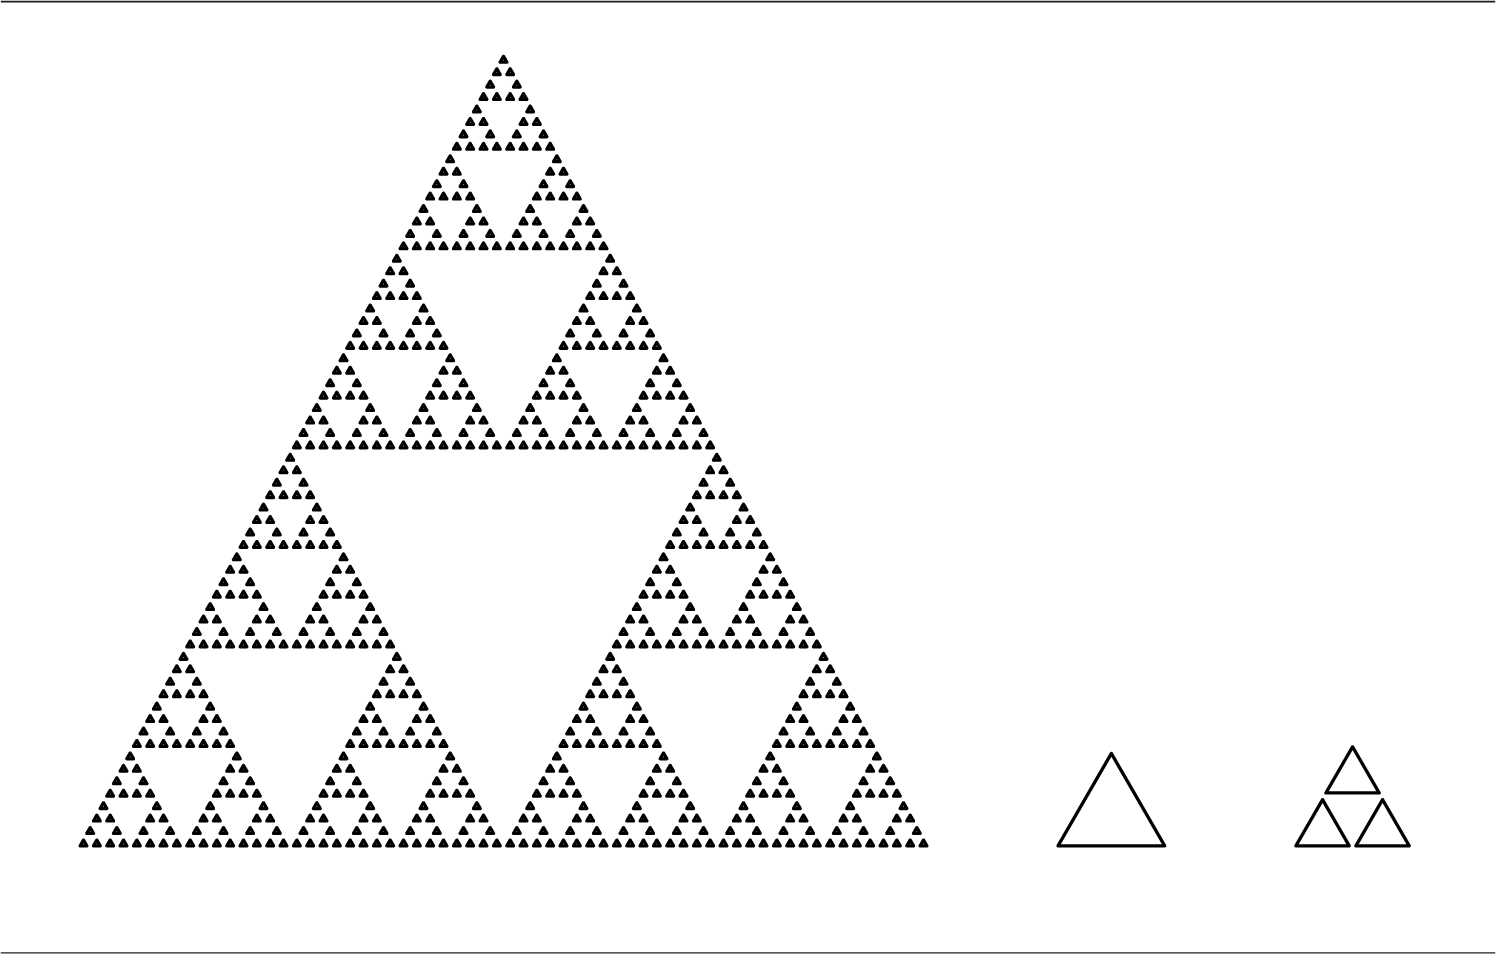
\includegraphics[width=0.8\textwidth]{images/00600.png}
  \caption{谢尔宾斯基三角形及其构造过程}
  \label{fig:sierpinski-triangle}
\end{figure}

图~\ref{fig:sierpinski-triangle} 最右侧的图像揭示了其生成步骤：给定一个大正三角形，找到各边的中点并将它们相互连结。这一步将大三角形划分为四个较小的全等三角形；只要小三角形的大小尚未达到视力或像素极限，就对除中心之外的三个外侧小三角形递归重复该过程。

另一种极为契合 \code{2htdp/image} 图像库组合函数的思路，基于从中间单三角形到右侧组合结构的过渡：将两个半尺寸的三角形水平并排（\code{beside}），然后在其上方居中放置一个相同的三角形（\code{above}），就能组合出大一号的双倍尺寸三角形：

\begin{lstlisting}[language=BSL]
(above half-sized
       (beside half-sized half-sized))
\end{lstlisting}

本节采用后一种自底向上的生成视角来设计谢尔宾斯基算法；第 34.3 节将使用前一种视角。由于目标是生成一个正三角形图像，我们用正数（三角形的边长 \code{side}）来表示该问题。这一决定给出了签名、目的说明与函数头：

\begin{lstlisting}[language=BSL]
; Number -> Image
; 生成边长为 side 的谢尔宾斯基三角形
(define (sierpinski side)
  (triangle side 'outline 'red))
\end{lstlisting}

现在我们来回答生成型递归的四个核心问题：
\begin{enumerate}
  \item \textbf{何为平凡问题？} 当给定的边长非常微小，以至于在其内部绘制更小的三角形已毫无意义时（例如小于阈值 \code{SMALL}），问题是平凡的。
  \item \textbf{平凡问题如何求解？} 此时只需直接画一个边长为 \code{side} 的基本正三角形即可。
  \item \textbf{如何生成新子问题？} 算法生成一个边长为 \code{side / 2} 的谢尔宾斯基三角形，因为三个这样的半尺寸三角形恰好能拼装出一个边长为 \code{side} 的新三角形。
  \item \textbf{如何合并子问题的解？} 若 \code{half-sized} 是边长为 \code{side / 2} 的谢尔宾斯基三角形图像，则表达式：
\begin{lstlisting}[language=BSL]
(above half-sized
       (beside half-sized half-sized))
\end{lstlisting}
  即为边长为 \code{side} 的谢尔宾斯基三角形。
\end{enumerate}

有了这些明确答案，定义函数便水到渠成。图~\ref{fig:sierpinski-code} 给出了完整实现。代码将平凡条件表达为 \code{(<= side SMALL)}，其中 \code{SMALL} 是一个预先定义的常数。在递归分支中，\code{local} 表达式引入局部变量 \code{half-sized} 保存递归调用生成的一半尺寸的谢尔宾斯基三角形，随后通过 \code{above} 和 \code{beside} 完成图元拼装。

\begin{figure}[htbp]
  \centering
\begin{lstlisting}[language=BSL]
(define SMALL 4) ; 像素级的微小尺寸阈值

(define small-triangle (triangle SMALL 'outline 'red))

; Number -> Image
; 生成型递归：生成边长为 side 的谢尔宾斯基三角形
; 方式：递归生成边长为 (/ side 2) 的半尺寸三角形，并将一个副本置于两个副本之上
(check-expect (sierpinski SMALL) small-triangle)
(check-expect (sierpinski (* 2 SMALL))
              (above small-triangle
                     (beside small-triangle small-triangle)))

(define (sierpinski side)
  (cond
    [(<= side SMALL) (triangle side 'outline 'red)]
    [else
     (local ((define half-sized (sierpinski (/ side 2))))
       (above half-sized
              (beside half-sized half-sized)))]))
\end{lstlisting}
  \caption{谢尔宾斯基三角形生成算法}
  \label{fig:sierpinski-code}
\end{figure}

最后进行终止性论证：\code{sierpinski} 的输入是一个正数 \code{side}。若该数值不大于正阈值 \code{SMALL}，算法直接终止；否则，递归调用接收的参数严格为当前边长的一半。只要初始边长与 \code{SMALL} 均为正数，连续除以 2 必然在有限步后进入小于等于 \code{SMALL} 的区间。因此该算法对于所有正数输入必然停机。

谢尔宾斯基算法的核心机制是：\textbf{不断将问题规模折半，直至可以直接求解}。稍加联想，你就会发现这种“区间折半”的过程可以用来极为高效地搜索满足特定性质的数值。下一节将深入剖析这一思想。

\section{二分搜索}
\label{sec:27_2}

应用数学家经常使用非线性方程对现实世界建模，并致力于求解这些方程。具体而言，他们将实际问题转化为从实数到实数的数学函数 $f$，并寻找某个实数 $r$ 满足：
\[ f(r) = 0 \]
这个数值 $r$ 被称为函数 $f$ 的\term{零点（root，或根）}。

\begin{notebox}[物理样例问题]
一枚火箭以 $v$ 英里/小时的恒定速度沿着直线向 $d_0$ 英里外的目标飞行。随后它以 $a$ 英里/小时$^2$ 的加速度加速飞行 $t$ 小时。火箭何时击中目标？
\end{notebox}

经典物理学告诉我们，火箭飞行的距离是时间的函数：
\[ d(t) = v \cdot t + \frac{1}{2} a \cdot t^2 \]
火箭击中目标的时刻就是剩余距离为 0 的时刻，即求解满足下式的 $t_0$：
\[ d_0 - \left(v \cdot t_0 + \frac{1}{2} a \cdot t_0^2\right) = 0 \]
初等代数告诉我们这是一个一元二次方程，在满足判别式条件时可用求根公式精确求解。

然而在工程实际中，问题往往远比二次方程复杂，很多方程根本不存在解析解。为此，数学家发展了多种针对不同连续函数的数值求根算法。本节探讨基于微积分早期核心定理——\term{介值定理（Intermediate Value Theorem, IVT，又称中间值定理）}的数值解法。这一算法是源自数学定理的生成型递归的典范。计算机科学家进一步将其推广为通用的\term{二分搜索（binary search）}算法。

\begin{notebox}[介值定理 (IVT)]
若实数函数 $f$ 在闭区间 $[a, b]$ 上是连续的，且 $f(a)$ 与 $f(b)$ 位于 $x$ 轴两侧（即一正一负，符号相异），则在区间 $[a, b]$ 内至少存在一点 $r$ 使得 $f(r) = 0$。
\end{notebox}

这里的“连续”直观上意味着函数图像是一条没有间断、跳跃和断裂的平滑曲线。图~\ref{fig:ivt-plot} 展现了介值定理的直观几何意义：函数 $f$ 在 $a$ 处位于 $x$ 轴下方，在 $b$ 处位于 $x$ 轴上方，因此其曲线必然在 $[a, b]$ 区间（图中标注为“range 1”）内横截穿过 $x$ 轴。

\begin{figure}[htbp]
  \centering
  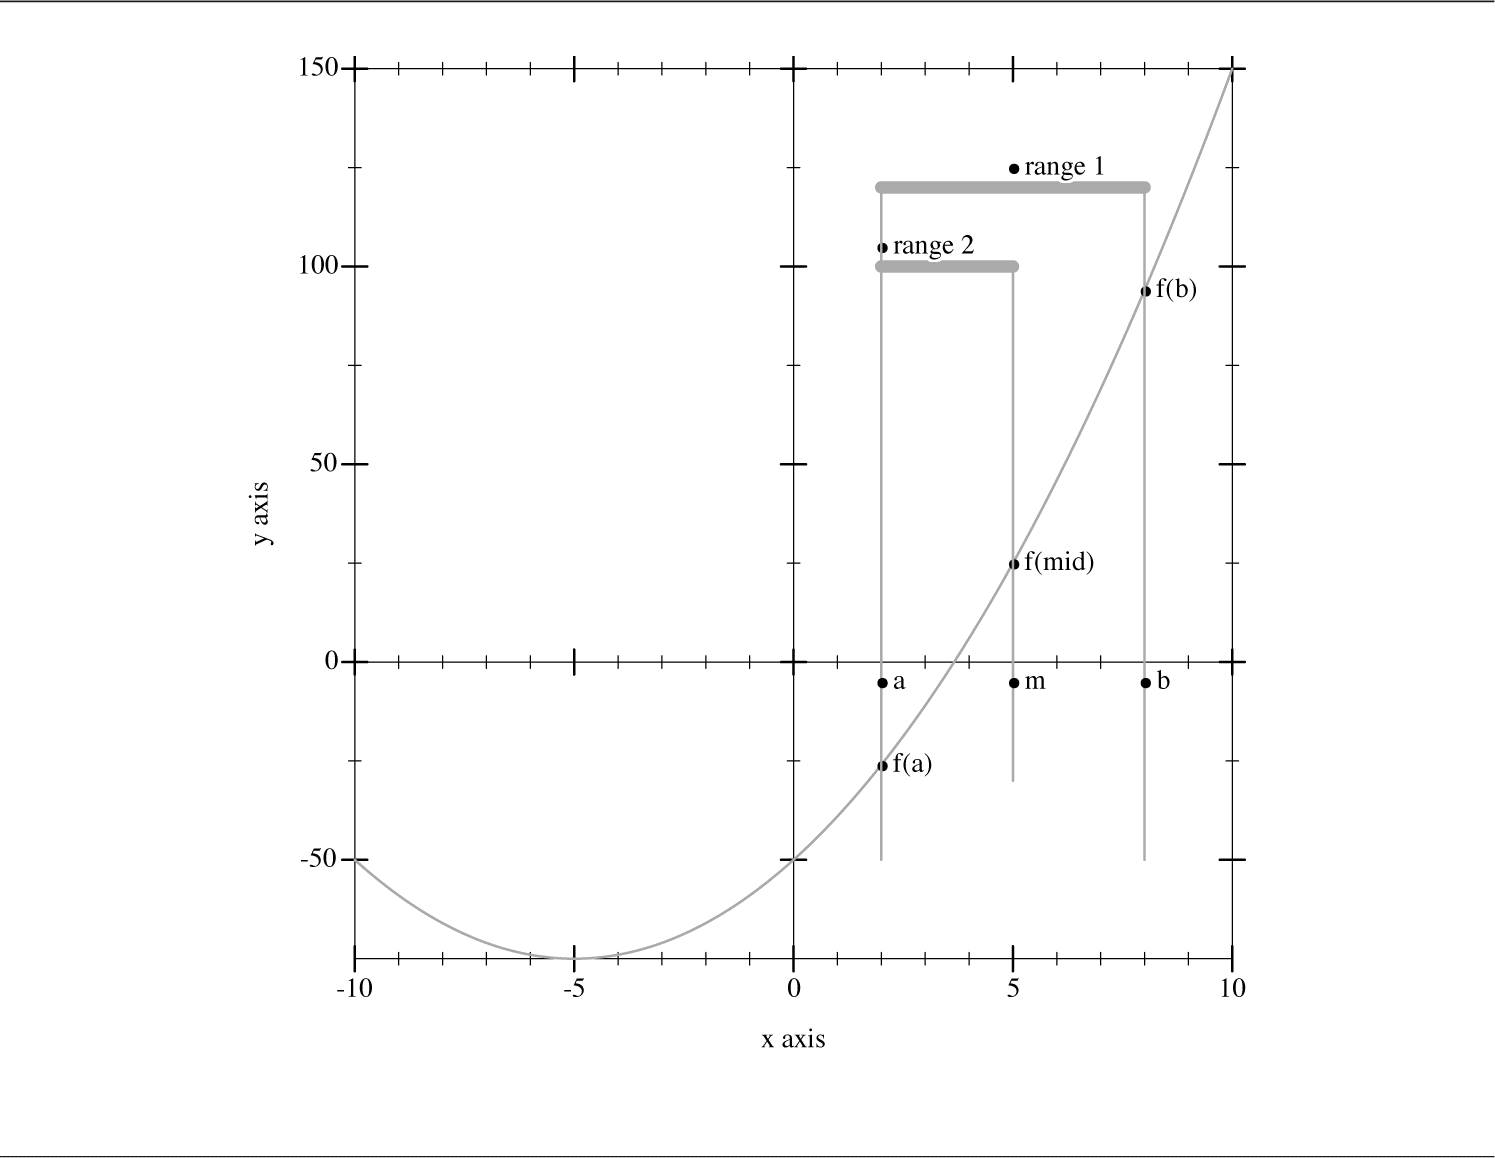
\includegraphics[width=0.8\textwidth]{images/00607.png}
  \caption{连续函数 $f$ 在区间 $[a, b]$ 内存在零点}
  \label{fig:ivt-plot}
\end{figure}

现在考察区间 $[a, b]$ 的中点（midpoint）：
\[ m = \frac{a + b}{2} \]
中点 $m$ 将大区间划分为两个长度减半的子区间：$[a, m]$ 与 $[m, b]$。计算中点处的函数值 $f(m)$：
\begin{itemize}
  \item 若 $f(m)$ 与 $f(a)$ 异号（即介值定理条件在左侧成立），则零点必定位于左半区间 $[a, m]$ 内（如图~\ref{fig:ivt-plot} 中的“range 2”所示）；
  \item 若 $f(m)$ 与 $f(b)$ 异号，则零点必定位于右半区间 $[m, b]$ 内。
\end{itemize}

我们现在有了求根核心步骤的清晰构想。接下来将其设计为 ISL+ 算法。算法接收一个数学函数以及预期包含零点的区间两端端点：

\begin{lstlisting}[language=BSL]
; [Number -> Number] Number Number -> Number
; 寻找 R 使得 f 在区间 [R, (+ R ε)] 内存在零点
; 前置假设 1：f 是连续函数
; 前置假设 2：(or (<= (f left) 0 (f right)) (<= (f right) 0 (f left)))
; 生成型递归：将区间折半，零点必在其中一半，依据假设 2 选择包含零点的那一半递归
(define (find-root f left right)
  0)
\end{lstlisting}

这里的 $\varepsilon$（可写为 \code{EPSILON}）是允许的误差阈值。随着搜索将区间不断折半，当区间跨度 \code{(- right left)} 缩小至不超过 $\varepsilon$ 时，搜索即告完成，此时返回区间的左端点 \code{left} 作为根的近似值。

\begin{exercise}{手算验证 poly 二项式求根}{445}\label{ex:445}
考虑多项式函数定义：
\begin{lstlisting}[language=BSL]
; Number -> Number
(define (poly x)
  (* (- x 2) (- x 4)))
\end{lstlisting}
这是一个二次函数，其解析根显然为 2 与 4。
\begin{enumerate}
  \item 利用 \code{poly} 为 \code{find-root} 设计一个基于 \code{check-satisfied} 的自动化测试。
  \item 以初始区间 $[3, 6]$ 和误差 $\varepsilon = 0$ 为例，按表格逐步记录二分求根的推演过程：列出每次迭代的 \code{left}、\code{right}、\code{mid}、$f(mid)$ 以及下一步选取的区间。
\end{enumerate}
\end{exercise}

针对算法设计的四个核心问题：
\begin{enumerate}
  \item \textbf{平凡情形判断}：当 \code{(<= (- right left) ε)} 时，区间跨度已在容差范围内，问题平凡解决。
  \item \textbf{平凡解}：直接返回当前的 \code{left} 端点。
  \item \textbf{生成子问题}：计算中点 \code{mid = (/ (+ left right) 2)} 及其函数值 \code{f@m = (f mid)}。若 \code{f(left)} 与 \code{f@m} 异号，生成左半区间 \code{[left, mid]}；否则生成右半区间 \code{[mid, right]}。
  \item \textbf{合并子问题的解}：子问题找到的根直接就是原问题的根，无需后处理合并。
\end{enumerate}

图~\ref{fig:find-root-code} 给出了 \code{find-root} 的完整实现。

\begin{figure}[htbp]
  \centering
\begin{lstlisting}[language=BSL]
(define ε 0.001)

; [Number -> Number] Number Number -> Number
; 确定 R 使得 f 在 [R, (+ R ε)] 内有根
; 假设 f 连续，且 f(left) 与 f(right) 在 x 轴两侧
(define (find-root f left right)
  (cond
    [(<= (- right left) ε) left]
    [else
     (local ((define mid (/ (+ left right) 2))
             (define f@mid (f mid)))
       (cond
         [(or (<= (f left) 0 f@mid) (<= f@mid 0 (f left)))
          (find-root f left mid)]
         [else
          (find-root f mid right)]))]))
\end{lstlisting}
  \caption{二分法求根算法}
  \label{fig:find-root-code}
\end{figure}

\begin{exercise}{验证 find-root 并在不同容差下实验}{446}\label{ex:446}
将练习~\ref{ex:445} 中的测试用例加入到图~\ref{fig:find-root-code} 的程序中。尝试不同的 $\varepsilon$ 取值（如 0.1, 0.001, 0.00001），观察近似结果精度的变化。
\end{exercise}

\begin{exercise}{包含两个零点的区间}{447}\label{ex:447}
多项式 \code{poly} 拥有两个零点（2 和 4）。如果在调用 \code{find-root} 时传入同时包含这两个零点的区间（例如 $[1, 5]$），函数会返回哪一个零点？为什么？
\end{exercise}

\begin{exercise}{find-root 的终止性论证与收敛速度}{448}\label{ex:448}
论证 \code{find-root} 对于所有满足前置假设的连续函数与初值必能停机。假设初始区间跨度为 $S$。第 $k$ 次递归调用时的区间跨度是多少？经过多少次递归调用后必有 $(- \text{right}\ \text{left}) \le \varepsilon$？
\end{exercise}

\begin{exercise}{消除函数值的重复计算与累加器雏形}{449}\label{ex:449}
仔细观察图~\ref{fig:find-root-code}：\code{find-root} 在每个阶段都对端点重复计算 $f$ 的值。例如在跨越递归调用时，若选择了 $[left, mid]$，下一次调用又会重新计算 $(f\ left)$。
\begin{enumerate}
  \item 先利用 \code{local} 消除同一次调用内部重复求值的问题。
  \item 进一步设计一个辅助函数：它不仅接收 \code{left} 和 \code{right}，还接收前一次计算好的 $(f\ left)$ 与 $(f\ right)$ 作为参数传递给下一步。
\end{enumerate}
这种随数值递归同步传递已计算结果的技术，就是第 VI 部分的主题——\term{累加器（accumulators）}。
\end{exercise}

\begin{exercise}{单调函数的二分求根简化}{450}\label{ex:450}
如果函数 $f$ 是单调递增的（即当 $a < b$ 时恒有 $f(a) \le f(b)$），请简化 \code{find-root} 中的符号判断逻辑。
\end{exercise}

\begin{exercise}{表结构的线性搜索与二分搜索对比}{451}\label{ex:451}
定义结构体 \code{table} 包含两个字段：长度 \code{length} 与函数 \code{array}。该函数接收自然数索引并返回对应数值：
\begin{lstlisting}[language=BSL]
(define-struct table [length array])
; Table 是结构体：(make-table N [N -> Number])
\end{lstlisting}
表检索辅助函数定义为：
\begin{lstlisting}[language=BSL]
; Table N -> Number
; 查询表 t 中索引为 i 的数值
(define (table-ref t i)
  ((table-array t) i))
\end{lstlisting}
表的零点索引是指满足 \code{(table-ref t i)} 最接近 0 的自然数 $i$。
\begin{enumerate}
  \item 设计 \code{find-linear}：对单调递增的表，使用从 0 递增到 \code{length} 的结构型递归进行\term{线性搜索}。
  \item 设计 \code{find-binary}：使用基于二分搜索的生成型递归快速定位零点索引，并为其撰写终止性论证。
  \item 设表长度为 1024，零点在 1023 处。分别计算 \code{find-linear} 与 \code{find-binary} 所需的查询次数。
\end{enumerate}
\end{exercise}

\section{解析初窥}
\label{sec:27_3}

计算机系统通过文件提供持久化存储。在我们的计算模型中，文件本质上就是一个包含单字符字符串（\code{1String}）的列表，其中夹杂着特殊的换行符：

\begin{lstlisting}[language=BSL]
; File 是以下之一：
; -- '()
; -- (cons "\n" File)
; -- (cons 1String File)
; 解释：表示文本文件的内容，"\n" 代表换行字符

; Line 是 [List-of 1String]
\end{lstlisting}

许多程序需要将文件按行处理。例如 \code{2htdp/batch-io} 库中的 \code{read-lines} 函数，其任务就是将如下格式的文件列表：
\begin{lstlisting}[language=BSL]
(list "h" "o" "w" " " "a" "r" "e" " " "y" "o" "u" "\n"
      "d" "o" "i" "n" "g" "?" "\n"
      "a" "n" "y" " " "p" "r" "o" "g" "r" "e" "s" "s" "?")
\end{lstlisting}
转换为由三行构成的列表：
\begin{lstlisting}[language=BSL]
(list (list "h" "o" "w" " " "a" "r" "e" " " "y" "o" "u")
      (list "d" "o" "i" "n" "g" "?")
      (list "a" "n" "y" " " "p" "r" "o" "g" "r" "e" "s" "s" "?"))
\end{lstlisting}

将离散的符号序列转换为结构化分层数据的过程称为\term{解析（parsing）}。实际应用中需要解析单词、数字以及语法树（词法分析与语法分析）。

对于将 \code{File} 转换为 \code{[List-of Line]} 的函数 \code{file->list-of-lines}，运用生成型递归的四个问题分析如下：
\begin{enumerate}
  \item 当文件为空列表 \code{'()} 时，问题平凡，返回 \code{'()}；
  \item 否则，文件包含至少一个字符或换行符。算法必须提取出首个换行符之前的所有字符作为“第一行”（\code{Line}）；
  \item 剥离掉首行及换行符之后剩余的部分构成同类的新子问题，递归调用 \code{file->list-of-lines} 予以解决；
  \item 最后，使用 \code{cons} 将第一行与剩余行列表组合起来。
\end{enumerate}

这一思路清晰表明我们需要两个结构型递归辅助函数：
\begin{itemize}
  \item \code{first-line}：收集遇到的第一个 \code{"\textbackslash n"} 之前的所有字符；
  \item \code{remove-first-line}：丢弃第一个 \code{"\textbackslash n"} 及其之前的所有字符，返回剩余文件内容。
\end{itemize}

图~\ref{fig:file-lines-code} 展示了完整代码。

\begin{figure}[htbp]
  \centering
\begin{lstlisting}[language=BSL]
; File -> [List-of Line]
; 将一个文本文件内容转化为行列表
(define (file->list-of-lines afile)
  (cond
    [(empty? afile) '()]
    [else
     (cons (first-line afile)
           (file->list-of-lines (remove-first-line afile)))]))

; File -> Line
; 提取文件首个换行符之前的所有字符
(define (first-line afile)
  (cond
    [(empty? afile) '()]
    [(string=? (first afile) "\n") '()]
    [else (cons (first afile) (first-line (rest afile)))]))

; File -> File
; 剔除文件第一行（包括换行符）并返回剩余文件
(define (remove-first-line afile)
  (cond
    [(empty? afile) '()]
    [(string=? (first afile) "\n") (rest afile)]
    [else (remove-first-line (rest afile))]))
\end{lstlisting}
  \caption{将文本文件转换为行列表的解析算法}
  \label{fig:file-lines-code}
\end{figure}

注意在 \code{file->list-of-lines} 中，传给递归调用的实参是 \code{(remove-first-line afile)}，绝非简单的 \code{(rest afile)}。由于每次至少移除了一个字符（或一行），子问题的文件长度严格缩短，因此算法必定停机。

\begin{exercise}{完善辅助函数的目的说明}{452}\label{ex:452}
为图~\ref{fig:file-lines-code} 中的 \code{first-line} 和 \code{remove-first-line} 编写规范、精准的目的说明与单元测试。
\end{exercise}

\begin{exercise}{分词器 tokenize 的设计}{453}\label{ex:453}
设计函数 \code{tokenize}，将一行字符（\code{Line}）拆分为记号（token）列表。在这里，记号要么是标点等单字符，要么是由连续小写英文字母组成的单词（\code{String}）。所有空白字符均被剔除。提示：参考 \code{string-whitespace?} 函数。
\end{exercise}

\begin{exercise}{矩阵构造函数 create-matrix}{454}\label{ex:454}
设计函数 \code{create-matrix}。它接收数字 $n$ 以及包含 $n^2$ 个数值的列表，生成一个 $n \times n$ 的嵌套列表矩阵。例如：
\begin{lstlisting}[language=BSL]
(check-expect
  (create-matrix 2 '(1 2 3 4))
  (list (list 1 2)
        (list 3 4)))
\end{lstlisting}
再编写至少两个测试用例，并运用生成型递归实现该函数。
\end{exercise}
